
\chapter{Methodology}
\begin{refsection}
This chapter discussed the research methods, procedures, and techniques that were used to systematically identify, select, process, and analyze information to address the specific problems posed in this study. It explained theorems, algorithms, and mathematical models employed, the materials and statistical tools that were used, the theoretical/conceptual framework, and the methods for analyzing data to ensure accurate interpretation of results.


\section{Research Design}
This study employed a Constructive Research Design, a methodological framework specifically utilized in Computer Science and software engineering to solve domain-specific problems through the creation of novel computational artifacts, algorithms, or mathematical architectures. Unlike descriptive or exploratory research that primarily observed existing phenomena, the constructive approach focused on the systematic development and rigorous validation of a proposed solution. This design dictated that the research had to yield a tangible, functional construct—in this case, an algorithmic framework—that addressed a defined technical gap, followed by an objective, mathematically grounded evaluation to prove the artifact's practical utility and theoretical soundness within the discipline.

In application to this study, observing or evaluating current design systems was insufficient to solve the "Generative Gap" and "Layout Fragility" identified in contemporary graphic design automation. Because existing industrial tools relied on static templates that caused destructive state management, solving this problem required the active construction of the ThemeSync orchestration architecture. By utilizing a constructive methodology, the researchers systematically engineered the tri-layer pipeline, integrating Graph Neural Networks (GNN) for spatial mapping with a Cassowary linear arithmetic solver and a Bi-directional State Machine for non-destructive, real-time recalculations. Furthermore, to bridge the gap between theoretical computation and practical application, the design integrated a mixed-methods evaluation paradigm. The framework's validity was established by first mathematically proving the artifact's structural integrity against a Heuristic Fitness Function, followed by a quantitative human-expert validation using a Mean Opinion Score (MOS) to guarantee professional aesthetic compliance.

\section{Theorems, Algorithms, and Mathematical Framework}
This section delineated the foundational theorems, computational algorithms, and mathematical models that drove the ThemeSync orchestration framework. Specifically, it formalized the underlying architecture of the Graph Neural Networks (GNN) utilized for probabilistically mapping spatial dependencies, alongside the Convolutional Neural Networks (CNN) deployed for quantitative aesthetic evaluation. Furthermore, this section explicitly defined the system of linear inequalities and objective functions governing the Cassowary constraint-solving algorithm, establishing the mathematical boundaries required to dynamically calculate optimal layout coordinates while strictly preserving user-defined geometric parameters.

\subsection{Perceptually-Consistent Color Quantization (K-Means Clustering)}
ThemeSync used K-Means Clustering in the CIE color space L*a*b, which is a perceptually uniform color space, unlike the non-linear RGB color space which is device-dependent, with the Euclidean distance between two points in the space directly proportional to the perceived difference between them by human vision.
The algorithm divided the number of pixels in a picture, n, into k color clusters by minimizing the \textbf{Within-Cluster Sum of Squares (WCSS):} as shown in the formula below:

\begin{center}
\begin{minipage}{0.8\textwidth}
\begin{equation}
J\ =\ \sum_{i\ =\ 1}^{k}\sum_{{\ x}_p\epsilon S_i}||x_p-\mu_i{||}^2
\end{equation}
\centering
%\textbf{Formula 1.} Within-Cluster Sum of Squares (WCSS).
\end{minipage}
\end{center}

The extraction process defines $x$ as the $L^*a^*b^*$ feature vector of an individual pixel, which is then grouped into clusters where $i$ represents the mean of pixels within a specific cluster $S_i$ \cite{Lertrusdachakul2025Hybrid}. These clusters ultimately determine $k$, the target color centroids representing the primary, secondary, and accent colors. By grounding the analysis in the $L^*a^*b^*$ color space, the system ensures that the resulting palette remains consistent across diverse display technologies; this is achieved because the Euclidean distance calculated between clusters through Formula 1 correlates directly with the visual difference perceived by the human eye \cite{Garcia2023}.

\subsection{Stylistic Marker Identification (SIFT/SURF)}
To ensure the conservation of specific institutional resources, such as the CSPC logo, the system employs Scale-Invariant Feature Transform (SIFT) and Speeded-Up Robust Features (SURF). SIFT extracts local keypoints that are resistant to scaling, rotation, and affine transformation \cite{Shaharom2023SIFT}. Mathematically, these keypoints are identified through a Difference of Gaussians (DoG) function as shown in Formula 2:

\begin{center}
\begin{minipage}{0.8\textwidth}
\begin{equation}
\mathbf{D}(x,y,\sigma)=(G(x,y,k\sigma)-G(x,y,\sigma))\ast \mathbf{I}(x,y)
\end{equation}
\centering
%\textbf{Formula 2.} Difference of Gaussians (DoG).
\end{minipage}
\end{center}

The application of Formula 2 allows the framework to recognize a logo in a high-resolution Master Design and accurately track its relative significance when transformed into heterogeneous formats \cite{Shaharom2023SIFT}. Furthermore, the framework utilizes SIFT/SURF to construct a mathematical Saliency Map of the inpainted background layer. In this computational pipeline, the inpainted background referred to a text-free base layer mathematically rebuilt from the borders of the master poster. In addition to this base layer, the system isolated specific stylistic markers—namely, the primary title artwork and decorative motifs (which were detected via YOLO and ranked by SIFT keypoint density)—to ensure these distinct visual assets were preserved and transferred to the target format. By aggregating the high-frequency keypoints detected via the DoG function---such as sharp gradients, dense textures, or disruptive visual noise---the system generates a spatial heat map. The orchestration engine subsequently utilizes this Saliency Map to calculate a Legibility Penalty, ensuring that dynamically injected text nodes are mathematically restricted from occupying visually noisy coordinate spaces.

\subsection{Linear Arithmetic Constraint Solving (The Cassowary Algorithm)}
The Cassowary Algorithm serves as the core engine for real-time layout optimization. It is optimized to solve systems of linear equalities and inequalities efficiently \cite{Jiang2020ORCSolver}. Every design element is represented by a set of variables: $x_i\left(left\right),y_i\left(top\right),w_i\left(width\right),h_i\left(height\right).$ Relational logic (e.g., margins and padding) is expressed through linear equations defined in Formula 3:

\begin{center}
\begin{minipage}{0.8\textwidth}
\begin{equation}
\begin{aligned}
x_{\text{logo}} &= x_{\text{boundary}} + 20 \\
x_{\text{right}} &= x_{\text{left}} + \text{width}
\end{aligned}
\end{equation}
\centering
%\textbf{Formula 3.} Linear Arithmetic Constraints
\end{minipage}
\end{center}

The solver uses a dual-simplex method to maintain these relationships established in Formula 3 incrementally, allowing the layout to re-calculate in milliseconds whenever a single variable—such as viewport width—is adjusted \cite{Li2024SMT}.

\subsection{Stateful Human-in-the-Loop Refinement}
The framework differentiates between two types of constraints based on mathematical priority to support real-time interaction \cite{Li2024SMT}:

\begin{enumerate}
    \item \textbf{Hard Constraints:} Manual user interactions, such as "nudging" a text box or locking a logo's position, are assigned infinite weight. These are strictly prohibited from being violated by the solver and are mathematically represented as a Hard Equality Constraint in Formula 4:

    \begin{center}
    \begin{minipage}{0.8\textwidth}
    \begin{equation}
    C_{\text{hard}} : f(x) = b
    \end{equation}
    \centering
    %\textbf{Formula 4.} Hard Equality Constraint
    \end{minipage}
    \end{center}
	
	\item \textbf{Soft Constraints:} Standard design rules (e.g., default margins) or suggested alignments are assigned finite weights ($w_i$). The solver attempts to satisfy these by minimizing the total error through a Weighted Objective Function defined in Formula 5:

    \begin{center}
    \begin{minipage}{0.8\textwidth}
    \begin{equation}
    \mathbf{minimize}\ \sum w_id_i\ 
    \end{equation}
    \centering
    %\textbf{Formula 5.} Weighted Objective Function
    \end{minipage}
    \end{center}
	
	Where $d_i$ represents the "slack" or distance from the target suggested state \cite{Penco2025LLM}.
\end{enumerate}

\subsection{Graph Neural Networks (GNN)}
The architecture of a Graph Neural Network (GNN) will be designed for processing relational data by maintaining and updating node states through a graph structure \cite{Wu2022GNN}. In the ThemeSync framework, the design canvas will be modeled as a graph structure. Each design element—such as a text block, logo, or image—will function as a node, while spatial and semantic relationships—such as alignment or proximity—will be represented as edges. Through a message-passing mechanism, nodes will exchange information with their neighbors, allowing the system to capture dependencies among elements. This process will enable the model to infer how design components will interact and depend on one another, supporting relational logic inference for layout optimization.

\subsubsection{Initial Feature Encoding}
Every design element will start with a set of basic information called a feature vector \cite{Zhou2020Review}. This initial description will record the element's spatial and visual properties, serving as the starting point for relational analysis as established in Formula 6:

\begin{center}
\begin{minipage}{0.8\textwidth}
\begin{equation}
h_i^{(0)}=\ [x_i,\ y_i,w_i,h_i,c_i,s_i] 
\end{equation}
\centering
%\textbf{Formula 6.} Initial Feature Encoding
\end{minipage}
\end{center}

In this formulation provided by the formula above, $(x_i, y_i)$ represents the specific position of the element on the canvas, while $(w_i, h_i)$ denotes its corresponding width and height dimensions. The term $c_i$ refers to the CIE $L^*a^*b^*$ color embedding extracted via K-Means clustering, and $s_i$ serves as the SIFT/SURF stylistic descriptor capturing the element's unique visual features. Because the baseline training dataset (CGL-Dataset) categorizes text under a generic supercategory rather than explicit semantic labels, the framework establishes visual priority through Implicit Geometric Hierarchy. During Dynamic Node Instantiation, the system algorithmically assigns Baseline Geometric Tensors (predefined bounding box dimensions, $w_i \times h_i$) to external administrative variables before they are encoded into the graph. The Graph Neural Network infers spatial dominance purely by evaluating these initial geometric parameters. Elements instantiated with a larger spatial footprint are mathematically assigned a higher relational weight by the GNN, ensuring they are positioned precisely at the top of the structural hierarchy without requiring explicit semantic tagging. By organizing these variables into the structure of Formula 6, the system creates a standardized input for the subsequent Graph Neural Network layers.

\subsubsection{Relational Inference via Message Passing}
The GNN will process these features through a layer-wise exchange \cite{Bronstein2023Geometric}. At each layer k, every element will compute messages from its neighbors to update its own representation as defined in Formula 7:

\begin{center}
\begin{minipage}{0.8\textwidth}
\begin{equation}
\begin{aligned}
m_{ij}^{(k)}\ =\phi(h_i^{(k)},\ h_j^{(k)},\ e_{ij}) \\
h_i^{(k+1)}=\psi(h_i^{(k)},AGG{m_{ij}^{(k)}:\ j\ \epsilon\ N(i)})
\end{aligned}
\end{equation}
\centering
%\textbf{Formula 7.} GNN Message Passing and State Update
\end{minipage}
\end{center}

In this architecture described by Formula 7, $\phi$ represents the message function, implemented as a multilayer perceptron (MLP) designed to compute pairwise relational features between adjacent nodes. The $\text{AGG}$ term denotes a permutation-invariant aggregation operator, such as mean or sum pooling, while $\psi$ serves as the node update function, utilized as a Gated Recurrent Unit (GRU) to update the hidden state of each node.

The connections $e_{ij}$ utilized within the message function of Formula 7 will carry edge features describing spatial logic, which are formally structured in Formula 8:
\begin{center}
\begin{minipage}{0.8\textwidth}
\begin{equation}
e_{ij}=\ [{\delta x}_{ij},{\delta y}_{ij},{IoU}_{ij},\ r_{ij}^{align}]
\end{equation}
\centering
%\textbf{Formula 8.} Edge Feature Vector
\end{minipage}
\end{center}

According to Formula 8, these features include distance, Intersection over Union (IoU), and an alignment score where 0 will mean no alignment and 1 will mean perfect alignment.

To optimize relational spatial logic, the Graph Neural Network (GNN) was trained to predict layout coordinates by utilizing the master design's structure as its initial input. During initialization, target elements that shared a semantic counterpart on the master layout (e.g., the logo row, header, and event details) were anchored at their counterpart's original positions, while unmapped elements were positioned in reading order between them; in the absence of a master layout, elements defaulted to a centered, naive stack. The model was trained on CGL-Dataset layouts from both initialization states, deliberately distorting the structure starts during training to simulate real cross-format mapping transformations. The final GNN output was registered back to the master's anchors, ensuring that the mapped elements retained their original placements while the network optimally placed the unmapped elements between them. On the held-out validation split, this structure-aware initialization reduced overall position error to 0.036 (compared to 0.050 for the structure start alone), and when registered to exact anchors, improved the placement of unmapped elements to a gap error of 0.075 versus 0.081 for standard linear interpolation.

\subsection{State Synchronization — Finite State Machine and JSON Schema}
The State Synchronization module will record every change the designer will make during a session. Each interaction — whether a position nudge, a resize, or an element lock — will be saved as an immutable entry in a JSON-based state chain  No prior state will ever be overwritten, which means the designer's complete editing history will be preserved and any earlier version of the canvas will be restorable.
Each designer action will be modeled as a state transition. When an action will be performed at time t, the system will move from the current canvas state St to a new state St+1 based on a deterministic transition function defined in Formula 9 

The State Synchronization module will record every definitive change the designer will make during a session. Each interaction—whether a finalized position nudge, a completed resize, or an element lock—will be saved as an immutable entry in a JSON-based state chain \cite{Sabau2024RealTime}. To ensure optimal computational latency, the state machine will operate strictly as an Event-Driven Post-Interaction Solver. The system will deliberately ignore continuous manipulation data (e.g., on-drag coordinate streams) to prevent overloading the solver pipeline. Instead, a state transition will only initiate upon a terminal user action. When a discrete event will be performed at time $t$, the system will move from the current canvas state $S_t$ to a new state $S_{t+1}$ based on a deterministic transition function defined in Formula 9 \cite{Kleppmann2022CRDT}.

\begin{center}
\begin{minipage}{0.8\textwidth}
\begin{equation}
S_{t+1}\ =\delta(S_t,e_t\ )\ 
\end{equation}
\centering
%\textbf{Formula 9.} State Transition Function
\end{minipage}
\end{center}

In the model represented by Formula 9, $S_t$ represents the current canvas state at time $t$, while $e_t$ denotes the specific, terminal interaction event performed by the designer (which includes on-drop coordinate shifts, on-resize-complete dimensional changes, lock toggles, and direct text edits.). The transition function is defined by $\delta$, which processes the current state and the discrete event to trigger the Cassowary recalculation and produce the subsequent stabilized state of the canvas.

Furthermore, to preserve the structural integrity of the append-only JSON state chain, undo and redo actions executed on the canvas did not rewrite or erase historical layout data; instead, they restored an earlier configuration by appending it as a newly generated state.   

After each transition, every affected element will be assigned a constraint type \cite{Liu2026Multimedia}. The classification logic for these elements is formally presented in Formula 10:

\begin{center}
\begin{minipage}{0.8\textwidth}
\begin{equation}
\begin{aligned}
c_i=Hard,\ if\ \ e_i\ will\ belong\ to\ U_{manual} \\
c_i=Soft,\ if\ \ e_i\ will\ belong\ to\ A_{algorithmic}
\end{aligned}
\end{equation}
\centering
%\textbf{Formula 10.} Constraint Classification
\end{minipage}
\end{center}

As specified in Formula 10, elements manually adjusted by the designer ($U_{manual}$) will be labeled as Hard constraints, meaning the system will not change their position or dimensions. Conversely, elements placed or adjusted by the algorithm ($A_{algorithmic}$) will be labeled as Soft constraints, which the system will be permitted to modify during layout optimization. 

\subsection{Validation of Hybrid Visual DNA Correctness}
To guarantee that the orchestration engine executes with absolute structural and stylistic precision, the framework will implement a dual-validation protocol to mathematically and programmatically ensure the correctness of the Hybrid Visual DNA prior to layout synthesis. Because the Visual DNA is composed of both extracted and injected variables, the validation will be bifurcated into Algorithmic Correctness and Administrative Correctness.

The correctness of the autonomously extracted color features will be mathematically validated by optimizing the Within-Cluster Sum of Squares (WCSS) during the K-Means execution, as established in Formula 3.1. To prevent the extraction of inaccurate or perceptual outlier colors, the algorithm will iteratively compute the WCSS across multiple centroid ($k$) configurations. The system will programmatically identify the optimal $k$-value by detecting the inflection point (Elbow Method) in the WCSS decay curve. This mathematical convergence will serve as the strict validation metric, guaranteeing that the extracted color centroids accurately and optimally represent the true perceptual variance of the master design template.

To prevent the typographic hallucinations inherent in traditional Optical Character Recognition (OCR) systems, the correctness of the user-defined typographic parameters (font family, font weight, and baseline geometric sizing) will be strictly enforced through pre-orchestration JSON Schema Validation. Prior to initializing the Graph Neural Network (GNN) or the Cassowary solver, the framework will parse the ingested Dynamic Content Payload against a rigid, predefined data schema. The validation algorithm verified that all inputs strictly conformed to programmatic constraints formalized via JSON Schema (Draft 2020-12). Specifically, typographic rules dictated that font weights belonged to a valid integer set $\in \{100, 200, \dots, 900\}$, and baseline font sizes were constrained between a minimum of 8 pixels and a maximum of 15\% of the viewport's shorter side. Furthermore, content payload rules required that every requested schema variable was present and formatted strictly as a string that did not exceed its predefined max_characters limit. If a user payload violates these structural boundaries, the system will programmatically reject the initialization, thereby guaranteeing deterministic typographic correctness and preventing downstream layout failure.

\subsection{Quantitative Layout Evaluation (Heuristic Fitness Function)}
To programmatically evaluate the structural and aesthetic validity of the generated coordinate layouts without relying on subjective human surveying, the framework implements a mathematically rigorous Heuristic Fitness Function. This objective function is formulated as a minimization problem, calculating an aggregate penalty score based on four distinct spatial constraints. The overarching fitness function is defined in \ref{formula:heuristic-fitness-function}:

\begin{center}
\begin{minipage}{0.8\textwidth}
\begin{equation}
\begin{aligned}
F_{layout} = \alpha P_{collision} + \beta P_{alignment} + \gamma P_{whitespace} + \delta P_{legibility}
\end{aligned}
\end{equation}
\centering
\label{formula:heuristic-fitness-function}
\end{minipage}
\end{center}

In Formula 11, the coefficients ($\alpha, \beta, \gamma, \delta$) represent static scalar weights empirically calibrated during Phase 3 testing to prioritize critical layout rules (e.g., $\alpha$ is assigned the highest weight to strictly penalize element overlap). The individual penalty variables are mathematically defined as follows:

\begin{enumerate}
    \item \textbf{Collision Penalty ($P_{collision}$):} This metric calculates the absolute area of spatial overlap between all independently generated bounding boxes ($B$). It ensures elements do not visually occlude one another, defined in Formula 12:

    \begin{center}
    \begin{minipage}{0.8\textwidth}
    \begin{equation}
    P_{collision} = \sum_{i=1}^{N} \sum_{j=i+1}^{N} Area(B_i \cap B_j)
    \end{equation}
    \centering
    %\textbf{Formula 12.} Collision Penalty
    \end{minipage}
    \end{center}
	
	\item \textbf{Alignment Penalty ($P_{alignment}$):} This metric calculates the spatial variance of generated nodes against a dynamically generated structural grid ($G$). It computes the minimum pixel distance from a node's baseline coordinate ($x_i$ or $y_i$) to the nearest gridline, defined in Formula 13:
    
    \begin{center}
    \begin{minipage}{0.8\textwidth}
    \begin{equation}
    P_{alignment} = \sum_{i=1}^{N} \min_{g \in G} | coordinate_i - g |
    \end{equation}
    \centering
    %\textbf{Formula 13.} Alignment Penalty
    \end{minipage}
    \end{center}

    The structural grid $G$ was dynamically constructed from the layout candidate's specific content area—spanning its margins, quarters, and center—and an element was evaluated as successfully aligned if its left edge, vertical center, or right edge directly intersected any established gridline. 

	\item \textbf{Whitespace Penalty ($P_{whitespace}$):} This metric evaluates the mathematical ratio of negative space to positive design elements, measuring its deviation from an optimal target ratio ($R_{target}$) established by the master template's visual DNA. It is defined in Formula 14:
    
    \begin{center}
    \begin{minipage}{0.8\textwidth}
    \begin{equation}
    P_{whitespace} = \left| \frac{Area_{canvas} - \sum_{i=1}^{N} Area(B_i)}{Area_{canvas}} - R_{target} \right|
    \end{equation}
    \centering
    %\textbf{Formula 14.} Whitespace Penalty
    \end{minipage}
    \end{center}

    For the whitespace ratio calculation, the reference area was strictly defined as the candidate's designated content region (e.g., the active text column within an art-column archetype) rather than the global page canvas. This localized area calculation ensured that asymmetric or split layouts were accurately evaluated for negative space without being inadvertently penalized for off-center spatial compositions.
	
	\item \textbf{Legibility Penalty ($P_{legibility}$):} This metric prevents text degradation by cross-referencing the predicted bounding boxes of text nodes ($B_t$) against the background Saliency Map ($S$) generated via SIFT/SURF. It calculates the sum of high-frequency visual noise pixels ($p$) underlying the text coordinates, defined in Formula 15:
    
    \begin{center}
    \begin{minipage}{0.8\textwidth}
    \begin{equation}
    P_{legibility} = \sum_{t \in TextNodes} \sum_{p \in B_t} S(p)
    \end{equation}
    \centering
    %\textbf{Formula 15.} Legibility Penalty
    \end{minipage}
    \end{center}

    By calculating these interconnected formulas, the orchestration engine mathematically discards invalid spatial configurations and exclusively presents layout candidates that approach the optimal $F_{layout}$ minimum.

\end{enumerate}


\section{Materials and Evaluation Methods}
This section outlined the comprehensive methodology utilized to construct, validate, and empirically evaluate the ThemeSync orchestration framework. It detailed the specific computational hardware, software environments, and foundational datasets required as the primary research instruments. Furthermore, this section defined the systematic procedures for both the automated algorithmic testing and the human-in-the-loop usability validation, alongside the targeted sampling techniques applied to the computational data. Finally, it established the precise statistical tools and overarching evaluation methods necessary to quantitatively measure algorithmic latency, constraint satisfaction rates, and user interaction efficacy, ensuring a rigorous and multi-dimensional assessment of the proposed architecture.

\subsection{Research Instruments and Data Gathering}
The primary instruments for this algorithmic study comprised specialized computational datasets and structured vector templates. These instruments provided the foundational data required to train the relational logic models and empirically test the real-time constraint solvers.

\subsubsection{Training Data and Feature Mapping}
To process visual layouts computationally and establish implicit spatial knowledge, the framework utilized the CGL-Dataset V2, which extends the foundational layout benchmark introduced by introduced by Li, Chen, Yi, Liu, Shen, and Wang [2023], which extended the foundational benchmark established by Zhou, Xu, Ge, Wei, and Xu [2022], as its primary offline training corpus. This dataset comprises 60,548 training and 1,035 test graphic design posters annotated across four structural supercategories: logo, text, underlay, and embellishment. This formalized corpus provided the requisite structural bounding boxes and spatial adjacency patterns necessary to train the Graph Neural Network (GNN) for relational layout inference. \cite{li2023radm, zhou2022cglgan}

Because the raw CGL-Dataset was structured in a tabular delivery format containing comprehensive administrative metadata (e.g., image\_id, file\_name, and nested annotations), the framework enforced a deterministic preprocessing pipeline prior to neural network ingestion. This preprocessing module systematically executed three distinct operations. First, the system performed noise reduction by programmatically discarding non-mathematical administrative columns to optimize tensor processing. Following this, the module executed JSON deserialization to unpack nested arrays within the annotations and text\_annotations columns, thereby extracting precise bounding box geometries (bbox) and baseline semantic identities (supercategory). Finally, the system performed saliency mapping by cross-referencing the extracted coordinate boundaries against the background saliency matrix (as illustrated in \ref{fig:cgl-visual-extraction}). This operation calculated a discrete numerical penalty weight, replacing the need to feed computationally heavy, raw spatial matrices directly into the GNN.

The culmination of this preprocessing pipeline yielded a structurally filtered node array, formatted precisely to populate the GNN's initial feature tensor ($h^{(0)}$). A representative sample of this structured training dataset, demonstrating both structural boundaries and extracted algorithmic features, was detailed in Annex~\ref{annex:cgl-node-array}.

\subsubsection{Emperical Master-Layout Dataset}
To resolve the domain transfer gap observed when applying generalized document layout models to authentic promotional graphics, an empirical dataset comprising 200 authentic graphic design master layouts was curated as a specialized research instrument. In this framework, a master layout represented any unflattened or rasterized visual composition containing institutional or event branding assets uploaded to initialize orchestration. While the CGL-Dataset V2 established baseline spatial intelligence, preliminary evaluations indicated that detectors trained exclusively on generalized e-commerce banners suffered from significant confidence degradation when deployed on real institutional event designs. Consequently, this curated domain-specific dataset served as the formal training and validation corpus for the Semantic Layout Parsing module.

The dataset encompassed 200 distinct, high-resolution master layout posters spanning academic, cultural, and organizational event domains. These graphical assets were collected from official institutional publication repositories and public campus organization channels under academic fair-use guidelines.

All 200 layout images were manually annotated using the Roboflow computer vision platform. To maintain taxonomic consistency across the pipeline, annotations strictly adopted the standardized four-class schema established by Zhou, Xu, Ge, Wei, and Xu [2022]: logo, text, underlay, and embellishment. The bounding box coordinates were delineated under formalized spatial boundary rules. To minimize annotator subjectivity and eliminate boundary drift, annotation tasks were distributed across independent annotators and subjected to systematic cross-validation audits. \cite{zhou2022cglgan}

The annotated corpus was partitioned using an 80/20 train-to-validation split, allocating 160 images to the training set and 40 images to the held-out validation set. Rigorous programmatic preprocessing and quality filtering were executed prior to model ingestion. A dedicated normalization pipeline standardized coordinate definitions to resolve mixed polygon and bounding box geometry exports. Furthermore, an area-threshold filter programmatically removed outlier bounding boxes whose spatial footprints exceeded 50\% of the total canvas area, preventing ambiguous background container boundaries from destabilizing anchor regression. Finally, an independent domain expert validated a representative 15-image stratified sample against formal class definition rubrics to confirm taxonomic accuracy prior to model training.

The resulting curated dataset was utilized directly to train the deployed layout detector (a YOLOv8s architecture initialized from COCO pretrained checkpoints and trained at 1024-pixel resolution). This dedicated dataset guaranteed that the perceptual parsing stage extracted structural bounding boxes with high confidence from authentic master layouts prior to graph construction and constraint solving.

\begin{figure}[H]
\centering
\begin{tabular}{cc}

\includegraphics[width=0.35\textwidth]{figures/Original.jpg} &

\includegraphics[width=0.35\textwidth]{figures/Inpainted.jpg} \\

(a) Original annotated layout &
(b) Inpainted background isolating the canvas \\[0.5em]


\includegraphics[width=0.35\textwidth]{figures/Saliency_Map.jpg} &

\includegraphics[width=0.35\textwidth]{figures/Saliency_Map_Sub.jpg} \\

(c) Saliency map output &
(d) Saliency map utilized for preprocessing \\
\end{tabular}

\caption{CGL-Dataset Visual Extraction Pipeline.} (a) The original annotated layout. (b) The inpainted background isolating the canvas. (c \& d) The corresponding saliency maps utilized by the preprocessing module to calculate the $P_{legibility}$ visual noise penalty weight prior to GNN ingestion.
\label{fig:cgl-visual-extraction}
\end{figure}

To guarantee deterministic execution and mathematical rigor, these preprocessed offline dataset arrays, alongside the runtime administrative typographic constraints defined in the Hybrid Visual DNA, were explicitly mapped to the mathematical variables established within the system architecture. \ref{tab:ingested-data-fields} demonstrated this precise correlation between the data structures and the algorithmic pipeline.

To adapt spatial coordinates across heterogeneous formats, the system mapped target elements to the master layout based on shared semantic roles (e.g., pinning the logo row and header, while omitting incompatible positional data such as a poster's title on an academic certificate). Target elements with matching roles were pinned to their original coordinate anchors from the master layout, and all remaining unmapped elements were positioned sequentially between them via linear interpolation. Following the Graph Neural Network's spatial refinement, the generated output was registered back onto these exact anchors, ensuring the final layout strictly preserved the master design's foundational structure.

While the offline dataset established the baseline spatial intelligence, the framework also required a secondary, dynamic data stream during runtime orchestration. Because the framework was specifically designed to handle distinct administrative domains—such as Identification Cards and Academic Certificates—the system was required to ingest the user's structural requirements prior to final coordinate calculation.

Rather than injecting hardcoded data records at this stage, the system ingested a structural schema. This lightweight JSON payload defined the expected structural classes of the variables (e.g., text nodes or repeating geometric groups). Crucially, to align with the GNN’s implicit geometric hierarchy, the schema explicitly assigned a Spatial Hierarchy Index to each variable. The Spatial Hierarchy Index instructed the Cassowary constraint solver to arrange nodes sequentially based on their predefined reading order (e.g., spanning from index 0 for the logo row down to index 8 for signature blocks on a certificate, or index 0 to 5 on an event ID). Rather than functioning as a direct size ranking, the index established each element's semantic role and vertical stack position. The system subsequently assigned a fixed baseline bounding box size to each specific role, ensuring that critical data points—such as the event title and attendee name—received the largest geometric dimensions regardless of their sequential placement A sample representation of this runtime schema payload, utilizing an academic certificate context, was structured and shown in Annex \ref{annex:dynamic-content-payload}:




To guarantee deterministic execution and mathematical rigor, both the preprocessed dataset arrays and the dynamic payload structures were explicitly mapped to the algorithmic variables established within the system architecture. \ref{tab:ingested-data-fields} demonstrated this precise correlation.

\begin{table}[ht]
\centering
\caption{Data-to-Algorithm Parameter Mapping}
\label{tab:ingested-data-fields}
\begin{tabular}{p{0.25\textwidth} p{0.22\textwidth} p{0.15\textwidth} p{0.22\textwidth}}
\hline
\textbf{Ingested Data Field} & \centering\textbf{Algorithmic Application} & \centering\textbf{Mathematical Variable} & \centering\textbf{Processing Module}\arraybackslash \\ \hline

\texttt{bbox [x, y]} 
& Top-left spatial coordinate 
& $(x_i, y_i)$ 
& GNN Initial Feature Encoding \\

\texttt{bbox [w, h]} 
& Baseline geometric tensor 
& $(w_i, h_i)$ 
& Implicit Geometric Hierarchy \\

\texttt{extracted\_ color\_centroids} 
& Algorithmic palette mapping 
& $c_i$ 
& Node Feature Aggregation \\

\texttt{administrative\_ typography (font\_family, weight)} 
& Strict brand typographic compliance 
& $S_i$ 
& Pre-Orchestration Schema Validation \\

\texttt{extracted\_ saliency\_weight} 
& Visual noise penalty metric 
& $p_i(\text{legibility})$ 
& Heuristic Optimization Loop \\

\texttt{spatial\_ hierarchy} 
& Tensor allocation priority 
& Placeholder Tensor 
& Dynamic Node Instantiation \\ \hline

\end{tabular}
\end{table}


\subsubsection{Synthetic Administrative Templates and Vector Assets}
To rigorously evaluate the framework's real-time orchestration engine, a controlled dataset of synthetic administrative templates was engineered. Rather than utilizing abstract graphic structures, these master files were explicitly modeled to represent high-constraint institutional domains, specifically Academic Certificates and event identification cards. The event identification cards were structured in an A6 vertical proportion and contained standardized fields including a logo row, an event title, an attendee name, and a designated role. These templates were programmatically structured as interconnected Scalable Vector Graphics (SVG) and JSON schemas, designed to encompass varying degrees of spatial complexity.

Crucially, these synthetic assets acted as the primary testing instruments to stress-test the Cassowary constraint solver. To simulate real-world Human-in-the-Loop (HITL) injection, the synthetic dataset generated dynamic payloads containing extreme spatial variables—such as unusually long string values for student names or maximum instantiation limits for repeating\_groups (e.g., signature blocks). This controlled injection validated the solver’s capacity to execute dynamic aspect ratio transformations, correctly enforce the mathematical spatial_hierarchy weights, and dynamically resize text elements without violating predefined bounding box limits or overwriting surrounding structural nodes.



\subsection{Research Procedure}
The algorithmic pipeline was executed in four distinct developmental phases, mapping directly to the proposed tri-layer orchestration architecture. This procedural approach ensured the systematic integration of the perceptual extraction models, the real-time constraint solvers, and the quantitative evaluation metrics.

\subsubsection{Phase 1: Data Extraction and Graph Construction}
In the initial phase, the Deterministic Style Extraction modules were programmed to autonomously parse master design templates. The system utilized K-Means Clustering and SIFT/SURF algorithms to mathematically isolate dominant color centroids and scale-invariant stylistic markers. Concurrently, the system executed Semantic Layout Parsing utilizing a YOLOv8s architecture for object bounding box detection—initialized from COCO pretrained weights and trained at a 1024-pixel resolution exclusively on the empirical master-layout dataset—alongside Tesseract OCR for text extraction, converting the flattened raster pixels into structured, editable nodes. Concurrently, the Graph Neural Network (GNN) architecture was constructed and trained using the CGL-Dataset. The GNN was trained to map these extracted visual elements into a formal mathematical graph, establishing the hierarchical node-edge dependencies and spatial reasoning baselines required for the layout generation.

\begin{figure}[ht]
    \centering
	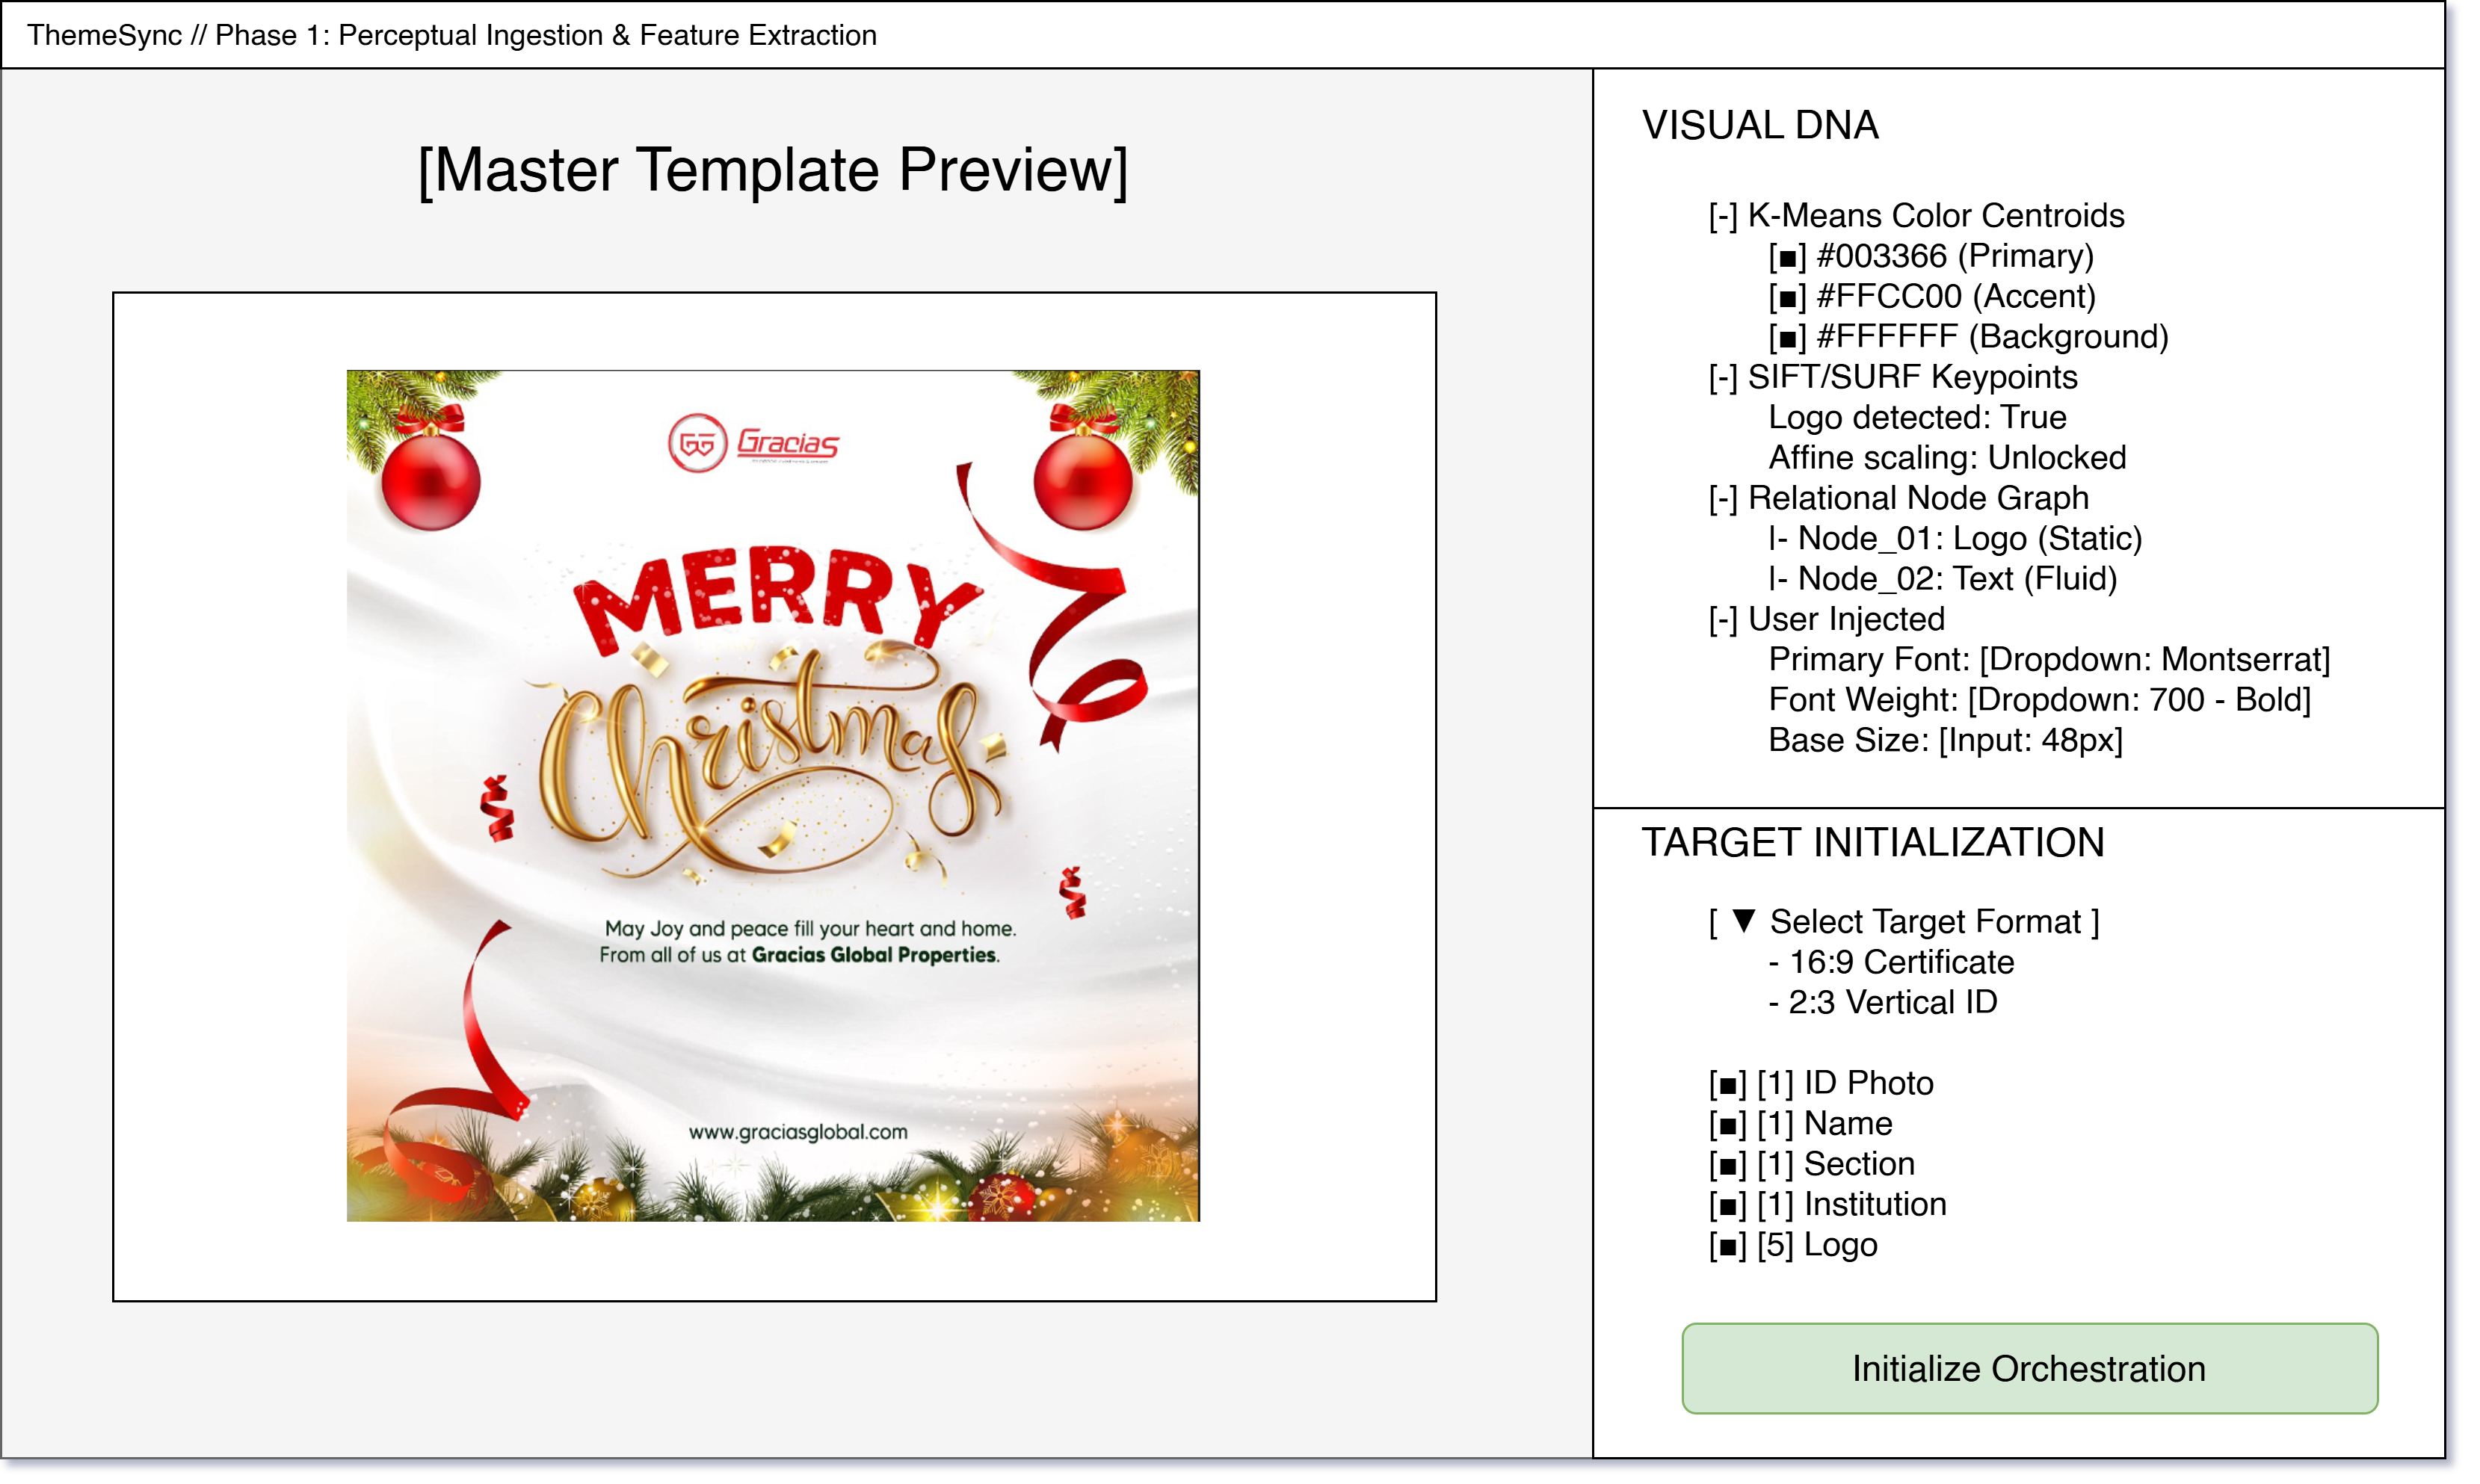
\includegraphics[width=0.85\textwidth]{figures/ts1.png} 
	\caption{Perceptual Ingestion and Initialization Dashboard.}
	\label{mockup:initializaiton-board}
\end{figure}

This interface (\ref{mockup:initializaiton-board}) demonstrated the initial data extraction and administrative configuration phase prior to layout synthesis. The central viewport displayed the uploaded master template, while the right-hand panel exposed the system's underlying mathematical diagnostics and input controls. This unified diagnostic panel explicitly presented the "Hybrid Visual DNA," logically partitioned into two components: the autonomous algorithmic extraction (including dominant color centroids identified via K-Means clustering, boolean feature detection via SIFT/SURF, and the structural hierarchy parsed by the GNN) and the administrative typography (where the user deterministically injected font families, font weights, and baseline geometric sizing). By allowing the designer to review the machine-extracted variables, define their strict typographic constraints, and select the target mathematical aspect ratio on a single workspace, the framework guaranteed that all necessary constraints and spatial boundaries were structurally established before initializing the orchestration engine.

\subsubsection{Phase 2: Constraint Satisfaction Problem (CSP) Integration and State Synchronization}
Following the construction of the relational graph, the second phase focused on real-time reactive layout synthesis. Prior to spatial calculation, the framework executed Dynamic Node Instantiation. The system ingested the user's Content Payload (external administrative datasets formatted as JSON) and algorithmically assigned Baseline Geometric Tensors to the new variables, establishing their Implicit Geometric Hierarchy within the graph. The Cassowary Algorithm was then mathematically implemented within the orchestration layer to act as the primary linear arithmetic constraint solver. Constraint equations were formulated and embedded to ensure bounding boxes dynamically adapted to varying aspect ratios without spatial overlap. Simultaneously, the Bi-directional State Machine was coded to serialize ongoing project states into lightweight JSON formats. This synchronization layer was explicitly programmed to capture manual user interventions from the Human-in-the-Loop (HITL) interface, translating them into hardened mathematical constraints to permanently prevent destructive overwriting during automated global updates.

\subsubsection{Phase 3: Heuristic Testing and Optimization}
The final procedural phase involved the rigorous testing and refinement of the generated coordinate layouts. The system was subjected to both the synthetic administrative templates and a testing battery of real, unseen event posters to execute parallel state-space explorations, effectively generating multiple layout candidates. The inclusion of authentic posters during this phase was strictly necessary because the calculation of the Legibility Penalty required a genuine visual background to accurately measure high-frequency visual noise and saliency. Specifically, these parallel explorations generated distinct candidates by varying four core compositional parameters: the structural layout archetype (e.g., classic centered, left-aligned, art column, or floating card), the page margin, the vertical rhythm governing the minimum gaps between stacked elements, and the decorative motif arrangement (such as diagonal, four corners, or a single enlarged hero motif). These algorithmic outputs were mathematically evaluated against the established heuristic Fitness Function. 

While the heuristic fitness function mathematically scored every generated candidate, the final recommended output was not determined solely by the lowest absolute $C_{total}$ penalty. Instead, the master layout's original visual composition dictated the target layout archetype (e.g., left-aligned text, an artwork column, or a footer band, defaulting to a classic centered structure in the absence of a master). The fitness function subsequently ranked the candidates within that mandated archetype to select the optimal output, ensuring the generation respected the source design's structural intent.

The system’s penalty weights—specifically the collision, alignment, whitespace, and Legibility penalties (derived from cross-referencing text coordinates against the SIFT/SURF Saliency Map)—were iteratively calibrated. This optimization loop continued until the mathematical scores demonstrated that the generated coordinate predictions consistently aligned with strict architectural constraints and human-centric design rules. Once the spatial coordinates were heuristically validated, the Aesthetic Rendering Pipeline executed. This final aesthetic rendering pipeline projected not only the K-Means color clusters and extracted stylistic typography onto the generated bounding boxes, but also the reconstructed background layer, the isolated decorative motifs, and the title artwork, thereby producing a fully populated and visually harmonized graphic layout.



\begin{figure}[H]
    \centering
    \begin{subfigure}{0.85\textwidth}
        \centering
        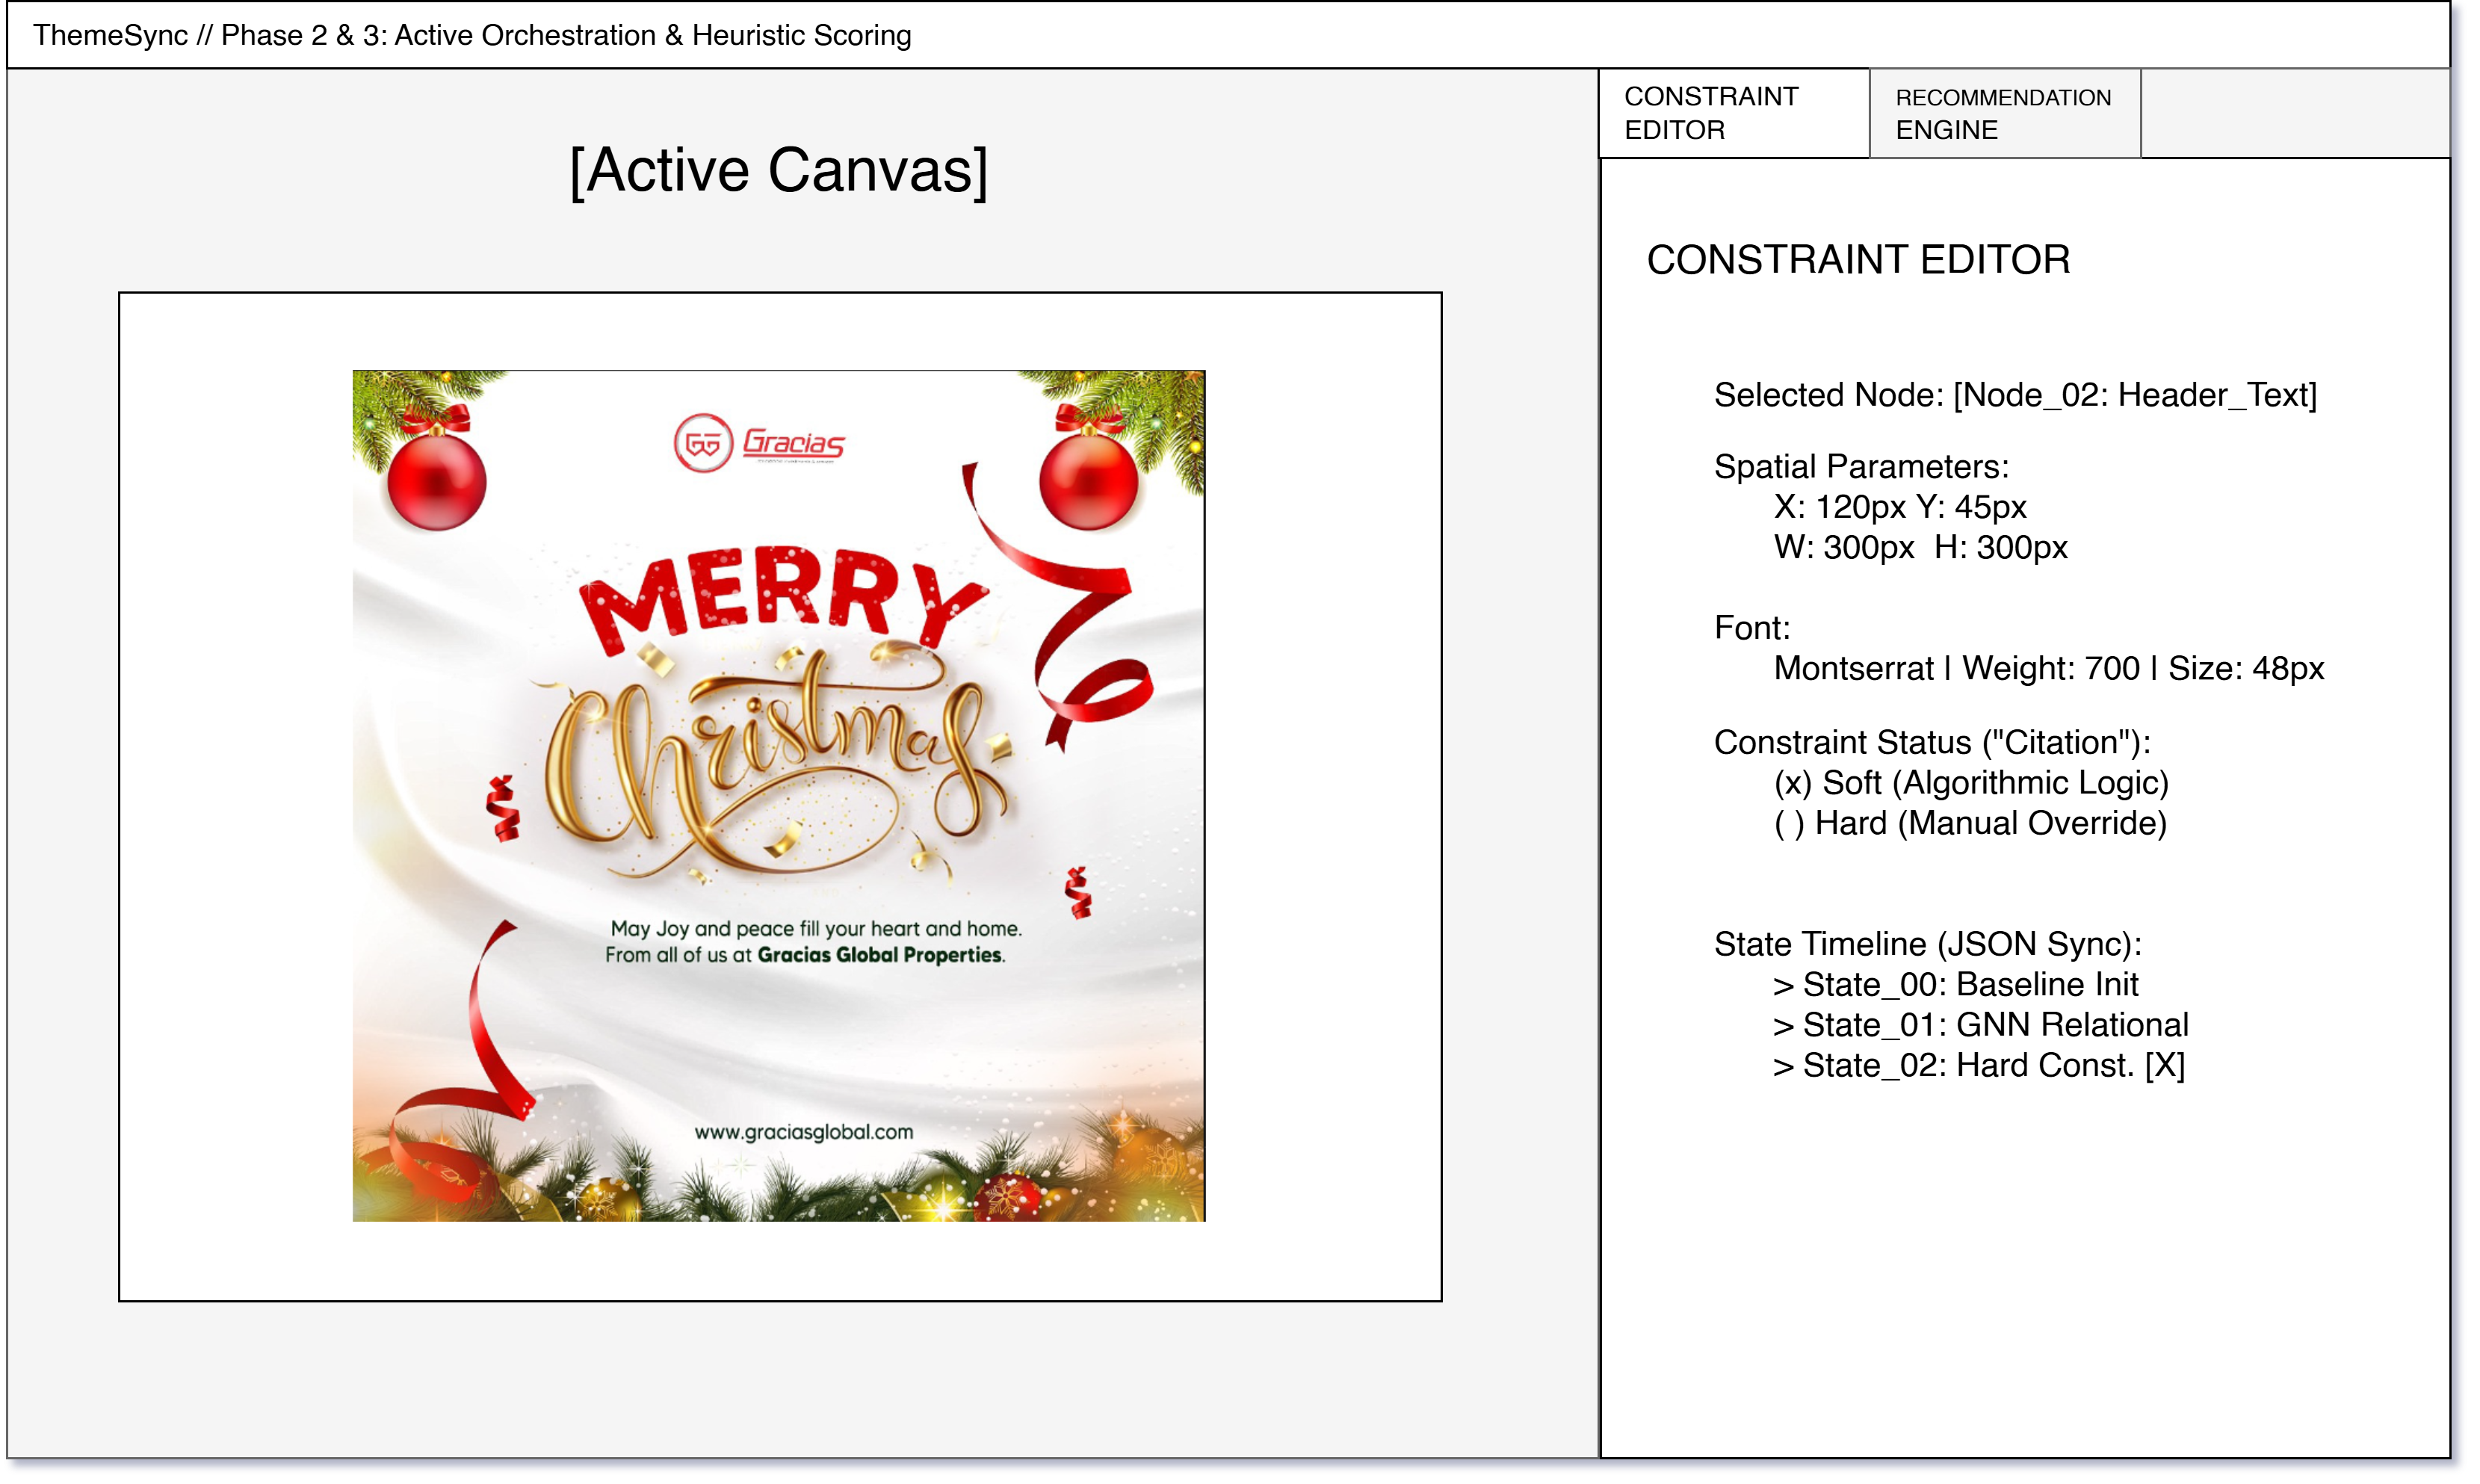
\includegraphics[width=\textwidth]{figures/ts2.png}
    \end{subfigure}

    \vspace{0.75cm}

    \begin{subfigure}{0.85\textwidth}
        \centering
        
\includegraphics[width=\textwidth]{figures/ts3.png}
    \end{subfigure}
    \caption{Active Orchestration and Heuristic Scoring Workspace}
    \label{mockup:active-orchestration-workspace}
\end{figure}

This unified workspace (\ref{mockup:active-orchestration-workspace}) illustrated the real-time execution of the Cassowary constraint solver, the schema validation protocols, and the aesthetic evaluation algorithms. The central canvas displayed the design adapting to the new target format. The right-hand interface was segmented into two critical computational tabs. The "Constraint Editor" tab exposed the solver's active parameters, displaying both the mathematical spatial coordinates (X, Y, W, H) and the schema-validated typographic parameters for the selected node. This allowed the designer to dictate whether specific elements were processed as algorithmic "Soft" constraints or mathematically locked "Hard" constraints. Below this, a serialized JSON timeline visually represented the Bi-directional State Machine, explicitly logging the successful Schema Validation of the user's typography and proving the non-destructive retention of manual user refinements. Concurrently, the Recommendation Engine displayed the generated candidates, where the underlying master layout's composition selected the appropriate layout archetype, and the heuristic fitness function ranked the specific variations within it.

The dashboard workflow formally concluded with a third step: a comprehensive Evaluation Report generated for the finalized layout. This report detailed the heuristic fitness calculation (\ref{formula:heuristic-fitness-function}) alongside the final recommendation, the structural accuracy (F1 score) per element, the manual edits retained through subsequent re-solves, stage and per-edit latency metrics, the K-Means elbow graph, and the schema validations.   

\subsubsection{Phase 4: Expert Aesthetic Validation}
Following the algorithmic generation and mathematical validation of the spatial coordinates in Phase 3, the orchestration framework underwent a final human-in-the-loop expert evaluation to ensure industry-standard aesthetic compliance. A panel of four designated domain experts—defined as professional layout artists and graphic designers with documented industry experience—interacted with the ThemeSync outputs. The deployment of multiple evaluators aligned with established usability and layout evaluation protocols \cite{nielsen1990heuristic, li2023radm, zhou2022cglgan}, which demonstrated that aggregating feedback from a minimum of three to five experts is required to reliably identify structural defects. The experts were tasked with reviewing a specifically designed experimental sample comprising 64 generated layouts. This evaluation set was derived from 16 unseen master layouts (event promotional materials explicitly withheld from the YOLOv8 training corpus) orchestrated across two target formats (Academic Certificates and event identification cards) under two distinct experimental conditions. To rigorously evaluate the framework's spatial intelligence, a blind no-GNN baseline condition was introduced. Layouts generated by the full ThemeSync orchestration engine were compared against baseline outputs generated with identical content but with the GNN module deactivated.

The resulting 64 layouts were compiled into printed evaluation packets, with each page displaying the original master layout alongside a generated candidate. To prevent evaluation bias, the generated layouts were assigned random sample codes, the page order was independently randomized for each expert, and pages derived from the same master layout were never placed adjacently. This evaluation sample size aligned with the established validation protocols of Zhou, Xu, Ge, Wei, and Xu [\citeyear{zhou2022cglgan}] and Li, Chen, Yi, Liu, Shen, and Wang [\citeyear{li2023radm}], which utilized 60-image test sets to validate generative layout models.

Rather than modifying the underlying computational architecture, the experts strictly evaluated the final visual outputs. They utilized a standardized Mean Opinion Score (MOS) rubric to quantitatively grade each generated layout. This evaluation measured critical design parameters that extended beyond absolute mathematical bounds, effectively bridging the gap between pure computational constraint satisfaction and subjective human design validity.

\subsection{Evaluation Metrics}
The validation of the orchestration framework utilized a mixed-methods approach. The core system architecture relied on controlled, quantitative metrics to measure algorithmic precision, spatial prediction accuracy, and computational efficiency. However, to ensure that the mathematically optimized layouts translated into viable professional designs, this rigorous computational benchmarking was followed by a structured, quantifiable evaluation by a panel of four human domain experts. This dual-validation methodology ensured that the framework achieved both mathematical constraint satisfaction and real-world aesthetic validity.

\subsubsection{Intersection over Union (IoU)}
Intersection over Union (IoU) was strictly confined to Phase 1 of the methodology to evaluate the extraction accuracy of the Semantic Layout Parsing module. During the initial ingestion of the Master Template, this metric calculated the area of overlap between the predicted bounding boxes generated by the YOLOv8 object detection model and the ground-truth annotations established in the empirical master-layout dataset's held-out validation split (40 images). By dividing the area of overlap by the area of union, the system yielded a strict, quantifiable score defining the exact geometric fidelity of the extracted nodes prior to relational mapping. Crucially, IoU was not utilized to evaluate the final dynamically generated layouts in Phase 3 or Phase 4, as orchestrating nodes across heterogeneous target aspect ratios inherently precluded the existence of a static ground-truth coordinate map.

\subsubsection{Algorithmic Latency}
This metric measured the time complexity and execution speed of the underlying algorithms, particularly the Cassowary Algorithm and the Bi-directional State Machine. Algorithmic latency was measured in milliseconds to mathematically demonstrate that constraint recalculations and state synchronizations executed within the strict time thresholds—specifically the 0.1-second limit for perceived instantaneous response and the 1.0-second limit for uninterrupted task flow—required for real-time Human-in-the-Loop (HITL) interface responsiveness. \cite{nielsen1993usability}

\subsubsection{Structural Accuracy Rate (F1-Score and Classification Metrics)}
The overall reliability of the reactive layout synthesis engine (Phases 2 and 3) was scored utilizing an F1-Score, derived from the harmonic mean of precision and recall. Because generating layouts for heterogeneous aspect ratios precluded the existence of a ground truth, the classification parameters for this metric were strictly mathematically defined by Constraint Satisfaction rather than spatial overlap.

A True Positive (TP) was recorded when the algorithm successfully generated and positioned bounding box coordinates for a required semantic node, provided that the node mathematically satisfied all designated constraints (i.e., it triggered zero collision penalties and strictly respected user-defined Hard Constraints).

Conversely, a False Positive (FP) was registered if the algorithm synthesized bounding box coordinates that violated a mathematically defined spatial boundary. This included invoking a collision penalty by overlapping an immutable designer-locked node, or protruding beyond the absolute dimensions of the target viewport.

Finally, a False Negative (FN) occurred when the algorithm completely failed to generate bounding box coordinates for a semantic node that was mathematically mandated by the Dynamic Content Payload or the relational graph of the master template, resulting in a missing structural element on the final design canvas.

\subsubsection{The Heuristic Fitness Function}
Layout evaluation was framed strictly as a mathematical optimization problem aiming to minimize the aggregate penalty score defined in Formula 11. The heuristic fitness function objectively scored parallel layout candidates by computing the Collision Penalty (Formula 12 to calculate overlapping nodal areas), the Alignment Penalty (Formula 13 to measure pixel variance from established gridlines), the Whitespace Penalty (Formula 14 to evaluate the mathematical ratio of negative space), and the Legibility Penalty (Formula 15 to quantify visual interference by cross-referencing text coordinates against the high-frequency keypoints of the SIFT/SURF Saliency Map). By utilizing these explicit mathematical thresholds, the framework guaranteed that subjective aesthetic principles were translated into rigorous, machine-readable metrics, thereby eliminating the necessity for subjective human surveying to validate structural accuracy.

\subsubsection{Mean Opinion Score (MOS) for Aesthetic Alignment}
To execute the expert aesthetic validation in Phase 4, the designated layout experts evaluated the generated multi-format layouts using a structured five-point Likert-type rating scale \cite{likert1932technique}. This Mean Opinion Score (MOS) quantified the subjective aesthetic validity of the final designs into rigorous, measurable data. The panel of experts evaluated the 64 generated layouts under both the GNN-guided and blind baseline conditions against three core design parameters:
\begin{enumerate}
    \item \textbf{Visual Hierarchy Preservation:} Evaluated whether the algorithmic coordinate placement maintained the correct structural dominance (e.g., ensuring a student's name or a certificate title visually remained the primary focal point relative to the surrounding nodes), serving as the subjective measure of visual emphasis. \cite{ODonovan2014Layouts}
    \item \textbf{Brand and Typographic Consistency:} Evaluated the framework's success in enforcing the Hybrid Visual DNA, specifically grading the accurate rendering of user-defined fonts, baseline geometric sizes, and algorithmically extracted color palettes without hallucination to ensure brand coherence. \cite{wheeler2013designing}
    \item \textbf{Constraint and Whitespace Harmony:} Evaluated the subjective quality of the spatial arrangement, confirming the visual absence of element occlusion (overlapping text/graphics) and verifying that the layout's negative space aligned with professional composition standard. \cite{ODonovan2014Layouts, zhou2022cglgan}
\end{enumerate}
Each of these qualitative parameters functioned as the human-evaluated counterpart to the system's internal computational metrics. While the implicit geometric hierarchy, the Visual DNA schema, and the heuristic fitness function (specifically Formulas 12 and 14) scored the layouts mathematically, the MOS evaluation verified that these strict computational bounds successfully translated into perceptually valid and aesthetically pleasing designs.

For each parameter, the experts assigned a numerical score based on the MOS rating scale shown in \ref{tab:mos-rating-scale}.
\begin{table}[ht]
\centering
\caption{Mean Opinion Score Rating Scale for Aesthetic Alignment}
\label{tab:mos-rating-scale}
\begin{tabular}{c p{0.28\textwidth} p{0.48\textwidth}}
\hline
\textbf{Score} & \textbf{Rating} & \textbf{Description} \\ \hline
5 & Excellent & No noticeable flaws \\
4 & Good & Minor aesthetic deviations \\
3 & Acceptable & Noticeable but non-destructive deviations \\
2 & Poor & Significant layout fragility \\
1 & Fail & Severe structural overlap or typographic failure \\ \hline
\end{tabular}
\end{table}
This rubric was adapted from the standard ITU-T P.800 Absolute Category Rating scale. To align with professional design evaluations, the standard midpoint "Fair" was renamed to "Acceptable," the baseline "Bad" was renamed to "Fail," and design-specific descriptive anchors were added to contextualize the grading criteria.

% \subsubsection{Statistical Treatment}
% To rigorously analyze the empirical data generated during both the computational benchmarking and the expert evaluation phases, the following statistical tools and procedures were employed:
% \begin{enumerate}
%     \item \textbf{Descriptive Statistics for Aesthetic Alignment:} In accordance with ITU-T Recommendation P.800 guidelines, the subjective evaluations gathered from the expert panel were aggregated by calculating the arithmetic mean and standard deviation. These descriptive statistics were computed for each of the three individual Mean Opinion Score (MOS) parameters, as well as for the overall layout quality.
%     \item \textbf{Inter-Rater Reliability:} To validate the consistency and consensus among the four independent domain experts, inter-rater reliability was measured using Kendall's Coefficient of Concordance ($W$). This non-parametric statistic was specifically selected to account for the ordinal nature of the five-point Likert-type rating scale.
%     \item \textbf{Comparative Significance Testing (MOS):} o determine if the layouts generated by the GNN orchestration engine represented a statistically significant aesthetic improvement over the blind no-GNN baseline condition, a Wilcoxon Signed-Rank Test was utilized. This test evaluated the paired ordinal samples for each master layout across both target formats.
%     \item \textbf{Comparative Significance Testing (Fitness Scores):} The quantitative heuristic fitness scores (Formula 11) logged between the GNN-guided and baseline configurations were similarly subjected to paired statistical difference testing to evaluate computational optimization improvements.
%     \item \textbf{Detection Accuracy:} The spatial prediction accuracy of the deployed Semantic Layout Parsing module was aggregated and reported as the mean Intersection over Union (IoU) across the 40-image held-out validation set.

\section{Theoretical and Conceptual Framework}
This section established the foundational theoretical principles and the overarching conceptual paradigm that governed the architecture and evaluation of the ThemeSync orchestration framework. It delineated the core computational theories underpinning the system, specifically drawing upon constraint-based layout theory to justify the mathematical resolution of spatial boundaries, alongside computational aesthetic theories to ground the machine-learning-driven evaluation models. Furthermore, this section presented the conceptual framework, explicitly mapping the systematic interaction of variables throughout the execution pipeline. It illustrated the continuous data flow from the initial ingestion of unstructured graphical layouts and user-defined parameters, through the concurrent processing of the neural network and mathematical modules, to the final output of stabilized, compositionally aligned design candidates. By synthesizing these theoretical and conceptual constructs, this section provided the rigorous academic scaffolding required to mathematically and logically justify the system's structural design and subsequent empirical methodology.

\begin{figure}[ht]
    \centering
	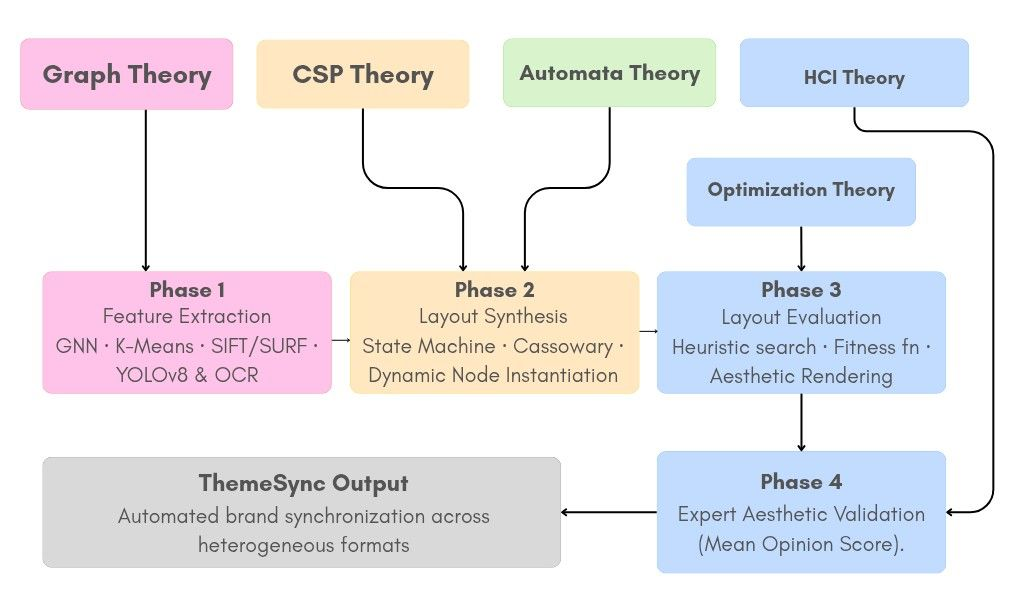
\includegraphics[width=0.85\textwidth]{figures/framework.jpeg} 
    \centering
    \caption{Theoretical Framework Diagram}
	\label{fig:theoretical-framework}
\end{figure}

\ref{fig:theoretical-framework} illustrated the theoretical framework that underpinned this research. The ThemeSync framework was grounded in five fundamental computer science theories: Graph Theory, the Constraint Satisfaction Problem (CSP) paradigm, Automata Theory, Human-Computer Interaction Theory, and Optimization Theory. These interconnected theoretical models provided the formal mathematical logic required to transition graphic layout orchestration from a static, coordinate-based generation task into a dynamic, stateful algorithmic pipeline.

\subsubsection{Graph Theory}
Graph Theory served as the primary theoretical basis for Phase 1 of the system, governing the relational logic of the layout components. In this context, a graphic layout was not modeled as a flattened array of pixels, but rather as a highly structured mathematical graph. Individual design elements, such as text blocks, image containers, and background shapes, operated as nodes, while the spatial and structural dependencies between them—such as proximity, alignment, and hierarchical nesting—operated as edges. This theory justified the application of Graph Neural Networks (GNN) and configurable graph-based frameworks within the system, establishing that deep learning models could accurately parse, traverse, and reconstruct the topological anatomy of a design by mathematically evaluating these node-edge relationships prior to rendering \cite{Wu2022GNN}. Furthermore, integrating perceptual extraction techniques, such as algorithmic palette mapping, directly into this graph ensured that stylistic and color identities remained mathematically consistent during structural transformations \cite{Kosarev2022Synthesis}.

\subsubsection{Constraint Satisfaction Problem (CSP) Paradigm}
The CSP paradigm underpinned Phase 2 by providing the theoretical basis for reactive layout synthesis. CSP defined problems where the state of a set of objects had to satisfy a specific number of logical or arithmetic constraints. Applied to spatial orchestration, responsive layout generation transformed into a complex equation-solving environment capable of supporting real-time GUI interactions \cite{Lukes2021WebLayouts}. Viewport dimensions and target aspect ratios were treated as mathematical variables, while structural rules and user intents were encoded as linear inequalities and adaptive OR-constraints \cite{Chen2024Gestalt}. This foundation governed the implementation of scalable constraint generation models \cite{Jiang2023LayoutFormer, MosqueiraRey2023HumanLoop}, proving that dynamic spatial harmony could be mathematically enforced in real time — eliminating the need for stochastic pixel placement.

\subsubsection{Automata Theory}
To address the persistent issue of destructive layout generation, the framework integrated principles from Automata Theory and state-machine logic. Automata Theory is the study of abstract machines and systems that transition between distinct computational states based on defined inputs. Within ThemeSync, this grounded the Bi-directional State Machine and its corresponding JSON schema handling. It provided the formal logical proof that the orchestration engine could maintain a persistent "memory" of localized manual edits—treating a user’s manual refinement as a highly specific computational state—and seamlessly transition the global template structure to a new iteration without irreversibly overwriting the human-in-the-loop modifications.

\subsubsection{Optimization Theory}
Optimization Theory supported Phase 3 of the system, governing the algorithmic evaluation of the generated layouts. Optimization Theory focuses on finding the best available mathematical solution from a massive set of feasible, parallel alternatives. In the context of automated orchestration, determining the optimal layout required navigating a rigorous mathematical search space. This theory justified the system's Heuristic Search mechanism, establishing that subjective aesthetic composition rules—such as geometric balance, whitespace distribution, and margin collision avoidance—could be quantified into objective penalty scores. By minimizing these penalty scores via a mathematical Fitness Function, the system successfully bridged the gap between automated spatial calculation and human-centric aesthetic validity.

\subsubsection{Human-Computer Interaction (HCI) Theory}
Finally, to support Phase 4, the framework drew upon Human-Computer Interaction (HCI) theory, which asserts that computational systems must align with human cognitive and perceptual standards to achieve practical utility. While Optimization Theory governed the mathematical minimization of spatial errors, HCI theory justified the necessity of the Mean Opinion Score (MOS). It provided the theoretical grounding that pure mathematical constraint satisfaction was insufficient for creative orchestration without human-in-the-loop validation. By structuring the expert’s subjective aesthetic evaluation into a quantifiable metric, the system proved that algorithmic layout generation could successfully synthesize mathematical precision with human-centric design expectations.



%=======================================================%
%%%%% Do not delete this part %%%%%%
\clearpage

\begin{center}
\textbf{Notes}
\end{center}
\printbibliography[heading=none]
\end{refsection}